\documentclass[a4paper,11pt]{report}
\usepackage[T1]{fontenc}
\usepackage[utf8]{inputenc}
\usepackage{lmodern}
\usepackage{graphicx}
\usepackage{url}
\usepackage{parskip}

% margins
\usepackage[top=2cm, bottom=3cm, left=3.8cm, right=3.8cm]{geometry}

% PDF file properties and links
\usepackage{hyperref}
\hypersetup{
  pdfauthor = {Sébastien Wilmet},
  pdftitle = {The GLib/GTK+ Development Platform},
  pdfcreator = {Texlive},
  pdfproducer = {Texlive},
  %colorlinks = false,
  pdfborder = 0 0 0
}

% Another package for code syntax highlighting is minted. By default minted has better colors for reading the document on a screen, but I think it is possible to have decent colors with listings too, it just requires more configuration. For printing purposes (without colors), I think listings is better. And this document is meant to be printed.
\usepackage{listings}
\lstset{
  language=C,
  basicstyle={\small\ttfamily},
  basewidth=0.5em,
  showstringspaces=false,
  captionpos=b
%   floatplacement=htbp
% Frames look nice, but it should be used cautiously. A frame around something means that the "something" is important. A frame will maybe be used later in this book to give a summary of important things. If each piece of code is surrounded by a frame, the important text will not be as highlighted as it should.
%   frame=single,
%   frame=tb,
% Will be useful later for large piece of code (create a new environment named lstlistinglarge or something like that).
%   linewidth=15cm,
%   xleftmargin=-1cm,
%   xrightmargin=-1cm
}

\lstloadlanguages{C, C++, Lisp, bash}

% Separate listings from the text (recommended in the Listings doc, instead of using frames).
% But with captions at the bottom, it is not very useful.
%\newcommand{\topfigrule}{\hrule\kern-0.4pt\relax}
%\newcommand{\botfigrule}{\hrule\kern-0.4pt\relax}

\newcommand{\shellcmd}[1]{\texttt{#1}}

\newcommand{\bookversion}{0.6}

\title{The GLib/GTK+ Development Platform\\[0.3cm]
{\normalsize A Getting Started Guide}\\[0.3cm]
{\normalsize Version \bookversion}}

\author{Sébastien Wilmet}

\begin{document}

\maketitle
\tableofcontents

\include{intro}
\include{glib}
\include{oop}
\include{oop-semi}
\include{oop-gobject}
\chapter{Example of a GTK+ Application Code Architecture}
\label{gtk-app-arch}

For any programming project, it is important to design correctly the general code architecture. With Object-Oriented Programming, it means defining the main classes. This chapter explains one example of a good code architecture for a GTK+ application, by looking at a simplified and a little enhanced view of the main classes of the gedit text editor\footnote{\url{https://wiki.gnome.org/Apps/Gedit}}.

gedit has a tabbed document interface; several files can be opened in the same gedit window, in different tabs. As we will see, this is reflected in the code architecture.

The Figure~\ref{fig:gedit-architecture} p.~\pageref{fig:gedit-architecture} shows the class schema. Every gedit class in the schema is a subclass of a GTK+ or GtkSourceView class. (GtkSourceView\footnote{\url{https://wiki.gnome.org/Projects/GtkSourceView}} is a library extending the \lstinline{GtkTextView} widget; \lstinline{GtkTextView} being part of GTK+.)

We will go through the class schema, explaining the classes step by step, by beginning at the top.

\begin{figure}
  \begin{center}
    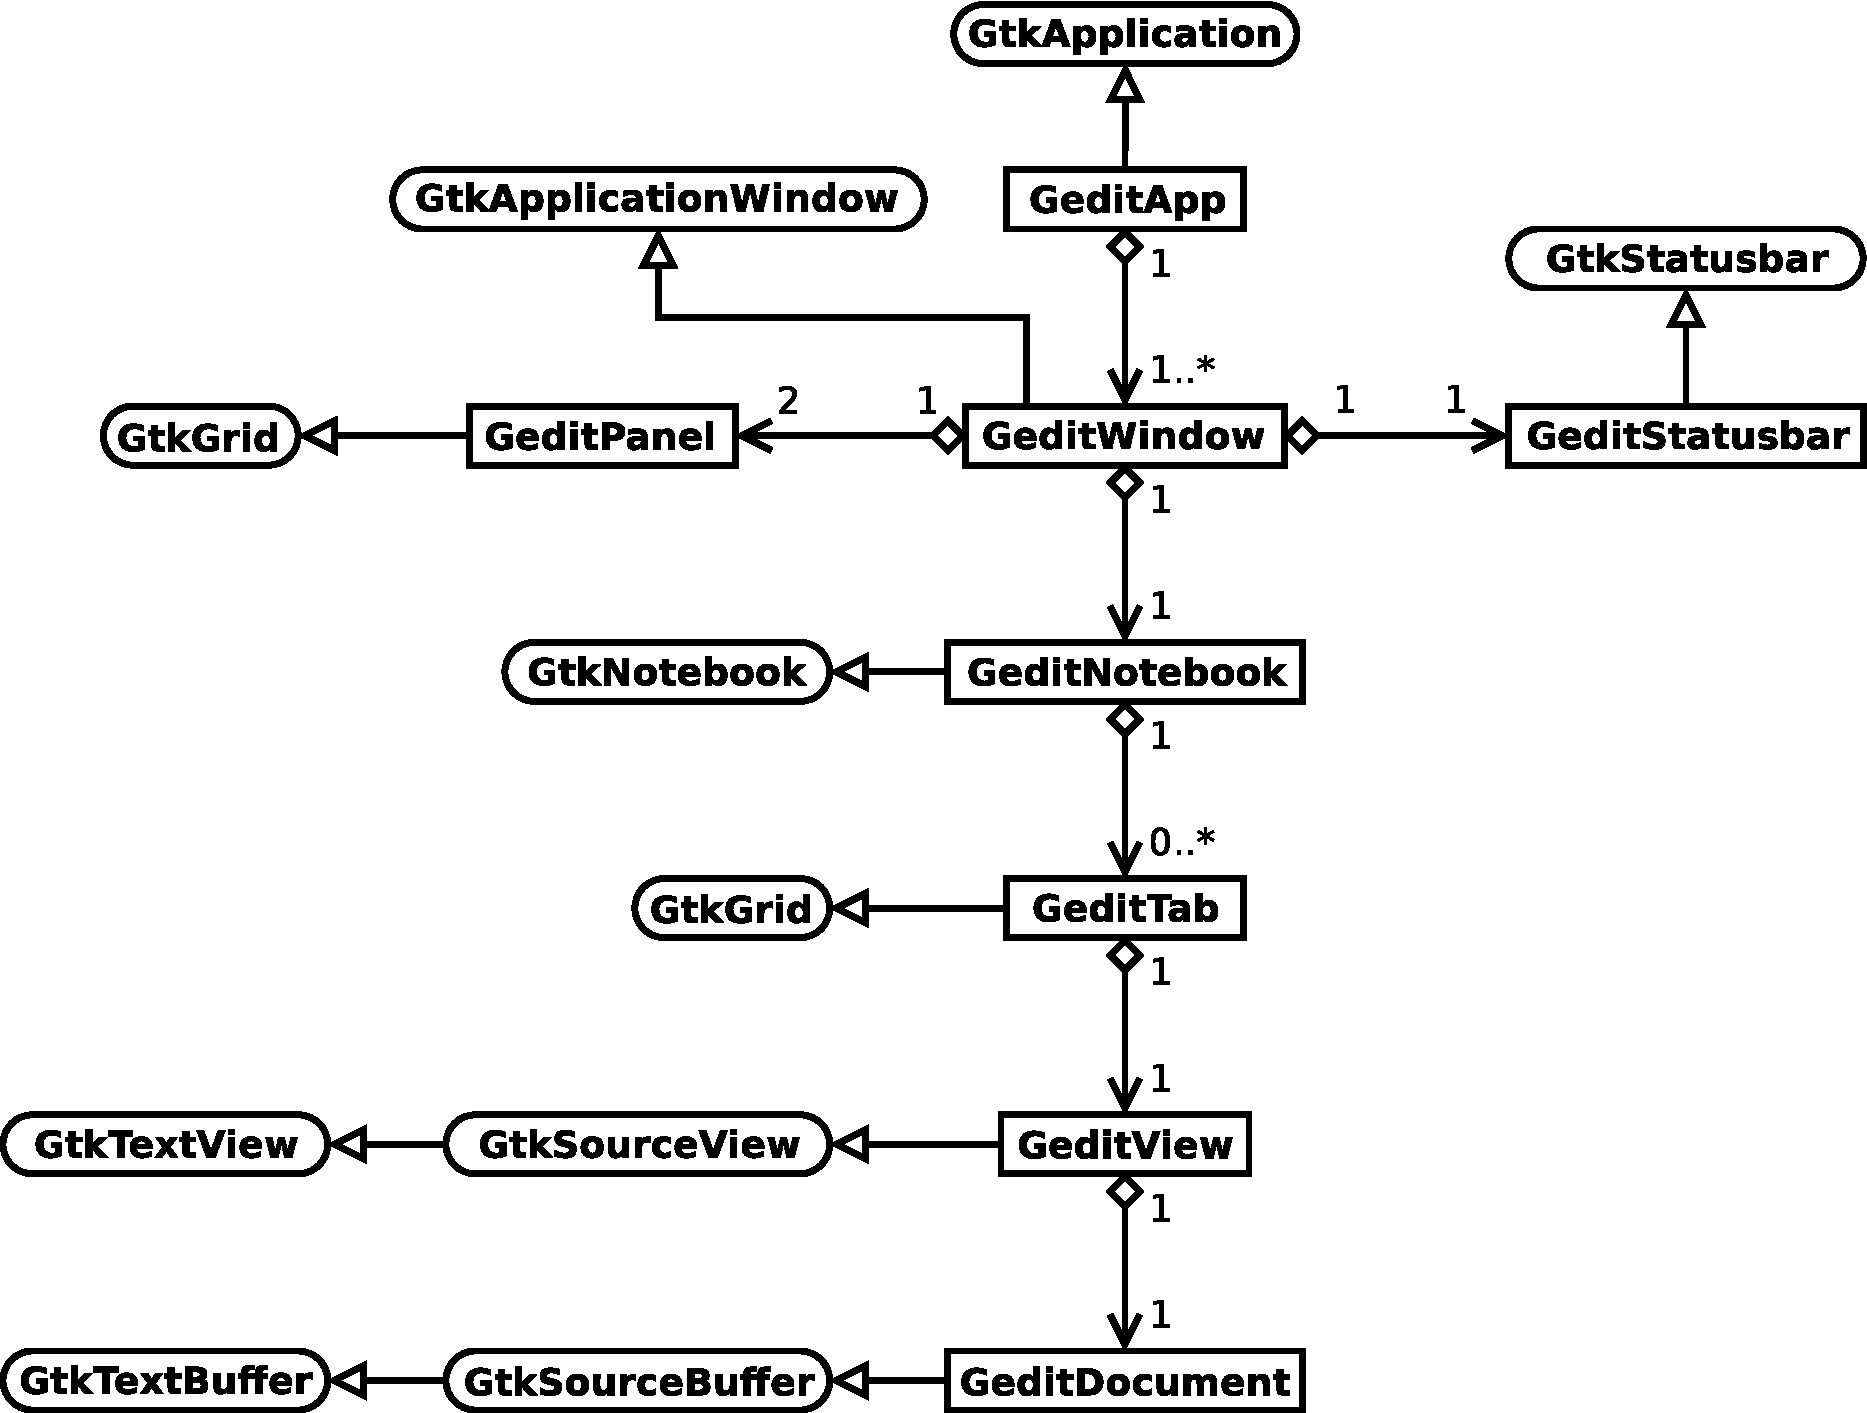
\includegraphics[width=\textwidth]{images/gedit-architecture.pdf}
    \caption{Simplified code architecture of the gedit text editor}
    \label{fig:gedit-architecture}
  \end{center}
\end{figure}

\section{GeditApp}

\lstinline{GeditApp} is a subclass of \lstinline{GtkApplication}. It is the class that contains and represents the whole application. There is only one instance of \lstinline{GeditApp}.

The \lstinline{main()} function of the program creates a \lstinline{GeditApp} instance instead of creating a \lstinline{GtkApplication} instance. What \lstinline{GeditApp} does is basically what you would need to do in \lstinline{main()} if there was no \lstinline{GtkApplication} subclass. This includes configuring the object correctly and connect callbacks to some signals (in a GObject subclass, instead of connecting callbacks to signals of the same class, it is better to override the virtual functions instead).

When you start writing a new GTK+ application, you don't see directly the need for a \lstinline{GtkApplication} subclass, since the code in \lstinline{main()}, plus the callbacks, are still small. But when more and more features are added, it is a good idea at some point to move the code to a \lstinline{GtkApplication} subclass.

\lstinline{GeditApp} is responsible to create the \lstinline{GeditWindow} objects when needed, for example on application startup, or when the user triggers an action that requires creating a new window. \lstinline{GeditApp} also implements the application-wide actions, with the \lstinline{GAction} API and related classes from the GIO library. An example of an application-wide action is to open the preferences dialog; because the preferences are applied to the whole application.

\section{GeditWindow}

\lstinline{GeditWindow} is a subclass of \lstinline{GtkApplicationWindow}. And, we don't see it on the schema, but \lstinline{GtkApplicationWindow} is a subclass of \lstinline{GtkWindow}, which is a top-level widget. A top-level widget cannot be contained in another widget. A \lstinline{GtkApplicationWindow} is contained in a \lstinline{GtkApplication}, but \lstinline{GtkApplication} is not a subclass of \lstinline{GtkWidget}.

In the schema, the ``\texttt{1}'' and ``\texttt{1..*}'' notation means that one \lstinline{GeditApp} object \emph{contains} one or several \lstinline{GeditWindow} objects, and that a \lstinline{GeditWindow} is contained in exactly one \lstinline{GeditApp} (a \lstinline{GeditWindow} cannot be contained in several \lstinline{GeditApp} objects, there is anyway only one \lstinline{GeditApp} instance per process).

\lstinline{GeditWindow} is responsible to create the main UI, creating other widgets and assembling them in a \lstinline{GtkGrid} container for example. Another thing that \lstinline{GeditWindow} does is to implement the \lstinline{GActions} that have an effect only on the current window, for example an action to close the window, or save the current document. When implementing a \lstinline{GAction}, \lstinline{GeditWindow} can of course delegate most of its work to other classes contained in \lstinline{GeditWindow}.

At the top of a main application window, there is usually a \lstinline{GtkHeaderBar}, that shows the window title, some buttons and an ``hamburger'' menu. Alternatively, an application can have a traditional menubar and toolbar.

Besides the headerbar, \lstinline{GeditWindow} creates a \lstinline{GeditStatusbar} widget and adds it to the bottom of the window. It also creates two \lstinline{GeditPanels}, one on the left side of the window, and the other on the bottom, above the \lstinline{GeditStatusbar}. Each panel can contain several elements. For example the side panel contains an integrated file browser, and the bottom panel can contain a terminal, among other things\footnote{The current gedit code actually doesn't contain a \lstinline{GeditPanel} class anymore, but it was the case in an earlier version. Adding \lstinline{GeditPanel} to the diagram was done to show a possible implementation of panels in an application. If your application contains only one element in a panel, no need to have a \lstinline{Panel} class, you can directly add the element to the window.}.

\lstinline{GeditWindow} also creates a \lstinline{GeditNotebook}, the main part of the window.

\section{GeditNotebook and What It Contains}

\lstinline{GeditNotebook} is a subclass of \lstinline{GtkNotebook}, which is the widget that displays tabs, and also contains their content.

In the class schema, we can see that the content of a tab is a \lstinline{GeditTab} widget, a subclass of \lstinline{GtkGrid}. The main element inside a \lstinline{GeditTab} is the \lstinline{GeditView}. More precisely --- it was omitted in the schema for succinctness --- the \lstinline{GeditView} is actually contained in a \lstinline{GtkScrolledWindow} which is contained in the \lstinline{GeditTab}. But \lstinline{GeditTab} can contain other widgets, for example information bars on top of the document.

\lstinline{GeditView} is a subclass of \lstinline{GtkSourceView}, which is itself a subclass of \lstinline{GtkTextView}. \lstinline{GtkTextView} --- which is part of GTK+ --- is the foundation for a multiline text editor. The GtkSourceView library adds features useful for source code, such as syntax highlighting. \lstinline{GtkTextView} follows a Model-View-Controller pattern. \lstinline{GtkTextBuffer} is the model, i.e. it contains the data.

\section{Why and When Creating Sub-Classes of GTK+ Widgets?}

If we look for instance at \lstinline{GeditTab}, it contains --- by composition --- a \lstinline{GeditView}. \lstinline{GeditView} is a subclass of \lstinline{GtkSourceView}. Instead, \lstinline{GeditTab} could use by composition directly a \lstinline{GtkSourceView} object, and move the code of \lstinline{GeditView} to \lstinline{GeditTab}. But usually, it's exactly the opposite that happens or should happen.

When a GTK+ application codebase is still small, for example if you start writing an equivalent of \lstinline{GeditTab}, you can create a \lstinline{GtkSourceView} object directly in \lstinline{GeditTab}, and store the \lstinline{GtkSourceView} object in an instance variable. Then, when implementing new features, you add new functions that use almost exclusively the \lstinline{GtkSourceView} instance variable. You may even have \lstinline{static} functions that take directly a \lstinline{GtkSourceView} argument instead of the \lstinline{GeditTab} \emph{self} parameter. You may also store additional data useful only to the \lstinline{GtkSourceView}-related functions. If the \lstinline{GeditTab} class is still small (e.g. 500 lines of code) and doesn't contain a lot of instance variables, there is no problem. On the other hand, if the \lstinline{GeditTab} class becomes larger (e.g. more than 2000 lines of code), then it's probably a sign that the class should delegate some of its work to a new class; in our case, \lstinline{GeditView}. Note that 2000 lines of code for a class might be fine, there is no clear boundary on when a class should be split. But if the resulting \lstinline{GeditView} class would contain at least several hundreds of non-boilerplate code, it is probably a good idea to do the refactoring.

What OOP is all about is to pack data and behavior together, and delegate some of the work to other classes. Class inheritance makes sense when we want to add more behavior to an existing class, with possible additional data related to the added behavior. \lstinline{GeditView} is a subclass of \lstinline{GtkSourceView} because \lstinline{GeditView} \emph{is~a} \lstinline{GtkSourceView}; that is, \lstinline{GeditView} operates on the same base data as \lstinline{GtkSourceView}. In addition, it permits to \lstinline{GeditTab} to delegate some of its work, with the goal to have smaller, more manageable classes. Smaller in two ways: less code, and less instance variables.

So, during the lifetime of a GTK+ application, the programmer often needs to refactor the code, creating new classes, delegating more work. The opposite can happen when application code is moved to the underlying library; for example, if all the features of \lstinline{GeditView} are added to the \lstinline{GtkSourceView} class; in that case, the \lstinline{GeditView} subclass doesn't make sense anymore.

\section{Composite Widgets}

Composite widgets are containers that already contain a useful collection of child widgets in a nice package. Implementing a composite widget is easy\footnote{Once you know how to subclass a GObject class.}, you just need to:
\begin{enumerate}
  \item Subclass a container like \lstinline{GtkGrid} or \lstinline{GtkBin} or \lstinline{GtkWindow};
  \item In the constructor of the class, create the child widgets and add them to the container.
\end{enumerate}

In the gedit class schema, the composite widgets are the subclasses of \lstinline{GtkGrid} (\lstinline{GeditPanel} and \lstinline{GeditTab}) and \lstinline{GeditWindow}.

\lstinline{GeditWindow} is an indirect subclass of \lstinline{GtkBin}, so it can contain at most one child widget. That's why \lstinline{GeditWindow} uses a \lstinline{GtkGrid} as its child widget, so that the \lstinline{GtkGrid} can contain in turn all the window elements.

By default a \lstinline{GeditTab} has only one child widget, the \lstinline{GtkScrolledWindow} that contains the \lstinline{GeditView}. But \lstinline{GeditTab} has a function to add a \lstinline{GtkInfoBar} at the top, showing for example an error message.

So, while \lstinline{GtkGrid} is a general-purpose container that doesn't contain any child widget initially, a composite widget is a specialized container that already contains specific child widgets. Writing composite widgets are a convenient way to code applications.

%TODO show code example

\include{further-reading}
\include{biblio}

\end{document}
